\documentclass{standalone}
\usepackage{amsmath}
\usepackage[T1]{fontenc}
\usepackage[utf8]{inputenc}

\usepackage[usenames,dvipsnames]{xcolor}

\usepackage{tikz}
\usetikzlibrary{arrows, shapes, matrix}

\begin{document}

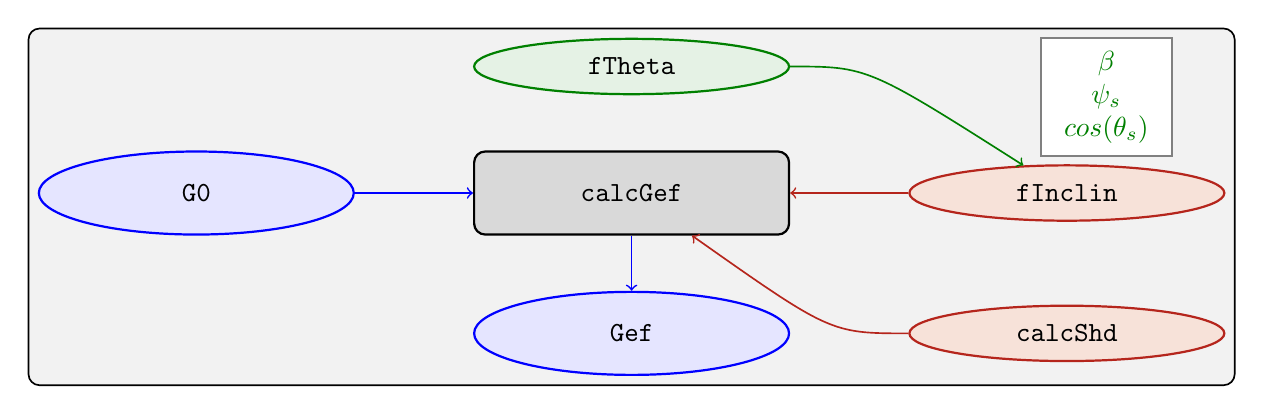
\begin{tikzpicture}[auto,
  method/.style={rectangle, rounded corners, draw=black, thick, fill=gray!30,
    minimum height = 3em, align=flush center, inner sep=1pt},
  %
  function/.style ={draw=BrickRed, thick, ellipse, fill=BrickRed!10,
    minimum height=2em},
  % 
  class/.style ={draw=Blue, thick, ellipse, fill=Blue!10,
    minimum height=3em},
  %
  utils/.style ={draw=Green, thick, ellipse, fill=Green!10,
    minimum height=2em},
  %
  simple/.style ={draw=black!50, thick, rectangle, fill=white}
  ]
  
  \tikzset{every path/.style={line width=.6pt}}

  \begin{scope}
    \matrix [matrix of nodes, rounded corners, fill=gray!10, draw=black, column
  sep=15mm,row sep=7mm, minimum width=4cm] (Geometry) {
    %%%%%%%%%%%%%%%%%%%%%%%%%%%%%%% 
    \node {}; &
    \node [utils] (ftheta) {\texttt{fTheta}}; &
    \node {}; \\
    %%%%%%%%%%%%%%%%%%%%%%%%%%%%%%%
    \node [class] (g0) {\texttt{G0}}; &
    \node [method] (calcgef) {\texttt{calcGef}}; &
    \node [function] (finclin) {\texttt{fInclin}}; \\
    %%%%%%%%%%%%%%%%%%%%%%%%%%%%%%%
    \node {}; &
    \node [class] (gef) {\texttt{Gef}}; &
    \node [function] (calcshd) {\texttt{calcShd}}; \\
  };
\end{scope}

\begin{scope}
  \draw [->, Blue] (calcgef) -- (gef);
  \draw [->, Blue] (g0) -- (calcgef);
  \draw [->, BrickRed] (finclin) -- (calcgef);
  \draw [->, Green] (ftheta) .. controls ++ (0:3) .. (finclin)
  node [simple, above, at end, xshift=3em, yshift=3pt] {$
    \begin{array}{c}
      \beta \\
      \psi_s \\
      cos(\theta_s)\\
    \end{array}
    $};
  \draw [->, BrickRed] (calcshd) .. controls ++(0:-3) .. (calcgef);
\end{scope}
  
\end{tikzpicture}

\end{document}
